\documentclass[aip, cp, amsmath, amssymb, reprint, nofootinbib]{revtex4-2}

\usepackage{graphicx}
\usepackage{dcolumn}
\usepackage{bm}

\input{preamble/preamble}
\input{preamble/tikz}
\input{preamble/macros}


% ========================================= %
% LaTeX Template by Aditya K. Rao
% Contact at adi.rao@mail.utoronto.ca

% Change for each document [!!!]
\newcommand\course{PHY426}	% Course Code [!!!]
\newcommand\doctitle{Investigation of Thin Lens Equation and Chromatic Dispersion} % Report Title [!!!]
\newcommand\firstauthorname{Aditya K. Rao} % Author Name [!!!]
\newcommand\firstauthorstdnum{Student Number: 1008307761} % Student Number [!!!]
\newcommand\firstauthoremail{adi.rao@mail.utoronto.ca} % Email [!!!]
%\newcommand\secondauthorname{Author Two}
%\newcommand\secondauthorstdnum{Student Number: 0000000000}
%\newcommand\secondauthoremail{report.author@mail.utoronto.ca}
\newcommand\advname{Tahir Shaaran\space} % Advisor Name [!!!]  
\newcommand\taname{Sean Crawford\space} % Advisor Name [!!!] 

\newcommand{\location}{MP222} % Location [!!!]
% ========================================= %
 
% ============== EQUIPMENT ================ %

\newcommand{\oscope}{\texttt{DSOX1202G}\space}
\newcommand{\pdiode}{\texttt{DET36A2}\space}
\newcommand{\hene}{\texttt{HNLS008L}\space}
\newcommand{\cam}{\texttt{Alium 1800 U-500}\space}

% ========================================= %

\usepackage{multirow}
\renewcommand{\arraystretch}{1.3}

%\pagenumbering{gobble}
\usepackage{listings}

\renewcommand\lstlistingname{Code Reference}
\renewcommand\lstlistlistingname{Code Reference}
\usepackage{tikz}
\usetikzlibrary{patterns}

\usepackage{circuitikz}

%\addbibresource{references.bib}
\usepackage{lipsum}
\usetikzlibrary{calc}

\begin{document}
\onecolumngrid
\pagenumbering{arabic}
\title{\doctitle}
\author{\firstauthorname}
\email{\firstauthoremail}
\thanks{\firstauthorstdnum}


%\email{report.author@mail.utoronto.ca}
%\thanks{Student Number: 0000000000}
\affiliation{
University of Toronto \\
\location, 60 St. George Street, Toronto, Ontario M5S 1A7, Canada.% Force line breaks with \\ if necessary
}

\date{\today} %Put in date of submission [!!!]

\preprint{APS/123-QED}
\begin{abstract}
    Multiple experiments were conducted to verify the thin lens equation for a variety of different lens types. The focal length of each lens was estimated through two methods. The first being a rudimentary estimation by point source far away and adjusting the lens until a focal point was found. The other by fitting and analyzing the thin lens equation and subsequent modifications. It was found that the thick lens equation represented the measurements better in all cases. However, the thin lens equation was still a good approximation for thin lenses. An additionaly experiment was also calibrated to characterized the chromatic aberrations in a plano-convex lens under different wavelengths of light.
\end{abstract}
    \maketitle
    %\tableofcontents 

    \lhead{\firstauthorname\vspace{0.1cm}}
    \chead{\textbf{\course} \\ \doctitle}
    \rhead{\textbf{Prof:} \advname \\ \textbf{TA:} \taname}
    \nocite{*}

    %\newpage
    \twocolumngrid
    \section{Introduction}
        % Plan
        % 1. Relavent Theory
        % 2. Simulation
        % 3. Talk about Hydrogen and Helium Emission Spectra, compare against lens data
        % 4. Talk about relavent theory for that
        % 5. Talk about the setup
        % Data Analysis and Relavent Results, make sure about unceratinties this time

        ptics and lesnes are a cornerstone of modern physics with their applications ranging from the study of the cosmos to the development of modern technology. In this experiment, the thin lens equation was quantiatively verified using a variety of lenses. The experiment was conducted in two parts. The first focused on verifying the thin lens equation, the second investigating if this still holds for thick lenses. Moreover, additional experimentation was conducted to investigate the diffraction patterns of light passing through a lens. Despite their significance, the foundational principles governing optical systems are often taken for granted. This experiment aims to rigorously test the thin lens equation through precise measurements using a variety of lenses.
        
        The experiment is divided into two main parts. The first focuses on verifying the thin lens equation and seeing if it may translate to thick lenses. The second extends this investigation into chromatic abberations in plano-convex lenses under different wavelengths of light.

        \subsection{The Thin \& Thick Lens Equations}
        
        The origins of the thin lens equation have been debated among historians. While the principles of lenses date back to ancient Greece, early mathematical formulations are often attributed to Isaac Barrow (1669) and Christiaan Huygens (1653) \cite{historyoptics}, who provided some of the first semi-verbal descriptions of the equation.
        
        \begin{equation} \label{eqn:thinlens}
            \frac{1}{f} = \frac{1}{p} + \frac{1}{q}
        \end{equation}
        
        Equation \eqref{eqn:thinlens} \cite{pwoptics} defines the fundamental relationship between the focal length of a lens ($f$), the object distance ($p$), and the image distance ($q$). A related equation \eqref{eqn:mag}\cite{pwoptics} describes the magnification ($M$) of an image.
        
        \begin{equation} \label{eqn:mag}
            M = -\frac{q}{p}
        \end{equation}
        
        Both equations assume that the lens is thin enough to be approximated by a two-dimensional plane rather than a three-dimensional object. In reality, a lens is better represented as having a front principal plane and a back principal plane (\figref{fig:real-lens}).
        
        \begin{figure}[H]
            %\input{figures/knife-edge.tex}
            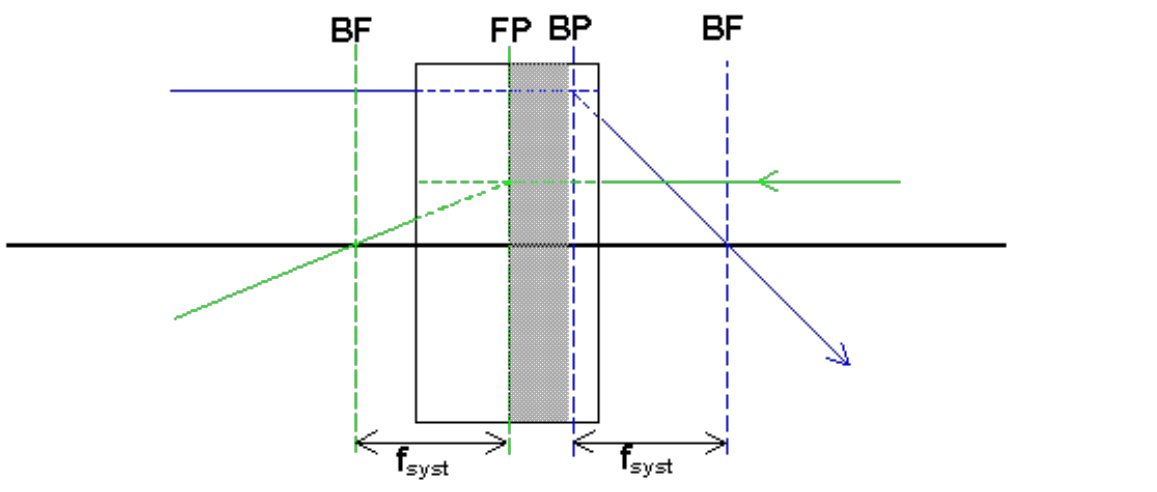
\includegraphics[width=0.8\linewidth]{figures/fp-bp.png}
            \caption{Illustration of principal planes in a real (thick) lens, adapted from the laboratory manual \cite{labmanual}. \texttt{BF} in the figure represents the back focal point, while \texttt{FP} and \texttt{BP} represents the front and back focal planes respectively. $f_\text{sys}$ is the system focal length.}
            \label{fig:real-lens}
        \end{figure}
        
        As can be seen in \figref{fig:real-lens}, there is indeed some ofset between the front and back principal planes. This offset is crucial in determining the focal length of a thick lens where this difference is exacerbated. Therefore, one may us \eqref{eqn:thicklens} \cite{pwoptics} to obtain a better approximation of the focal length of a thick lens.

        \begin{equation} \label{eqn:thicklens}
            \frac{1}{f} = \frac{1}{|o-l|-f_p} + \frac{1}{|i-l|-b_p}
        \end{equation}
        
        Where $p_f$ and $p_b$ are the distances from the front and back principal planes to the object and image respectively. $p = |o-l|$ and $q = |i-l|$ are the distances from the object and image to the lens respectively. Then,  thin lens equation is just a special case of \eqref{eqn:thicklens} with $p_f = p_b = 0$.

        \subsection{Chromatic Aberrations}
        
        Lenses in practical applications rarely behave as ideal thin lenses due to inherent optical imperfections. These deviations, known as aberrations, can significantly affect image quality. In general, there are five primary Seidel aberrations including \textit{spherical aberration}, \textit{coma}, \textit{astigmatism}, \textit{field curvature}, and \textit{distortion}. These aberrations can be further classified into two categories: geometric and chromatic. Additional study was specifically conducted \textit{chromatic aberrations}, or coma, which occur as a result of light dispersion within the optical matieral of the lens. The dispersion relation for a dielectric material is given in \eqref{eqn:dispersion}.

        \begin{equation} \label{eqn:dispersion}
            n^2(\omega) = 1 + \frac{N^2}{\varepsilon_0 m _e}\frac{1}{\omega_0^2 - \omega^2}
        \end{equation}

        Which may further be reduced \cite{labmanual} to \eqref{eqn:dispersion2} to solve for $\omega$.

        \begin{equation} \label{eqn:dispersion2}
            \frac{1}{n^2 - 1} = \frac{C}{\lambda_c^2} - \frac{C}{\lambda^2} 
        \end{equation}

        Where $C$ and $\lambda_c$ are constants for the material and $\lambda$ is the wavelength of the light, and $n$ is the refractive index. For air, this may be calculated using the len's maker equation \eqref{eqn:lensmaker}.

        \begin{equation} \label{eqn:lensmaker}
            \frac{1}{f} = (n-1)\left[\frac{1}{R_1} - \frac{1}{R_2} + \frac{(n-1)d}{n R_1 R_2}\right]
        \end{equation}

        Where $R_1$ and $R_2$ are the radii of curvature of the lens and $d$ is the thickness of the lens. 

        Specifically, for this section of the experiment, the change in the focal length of a plano-convex lens was measured under different wavelengths of light (i.e. different colors). These results were compared to a known wavelength as calculatd by a triprism spectroscope with calibration equation given in \eqref{eqn:triprism} \cite{labmanual}.

        \begin{equation} \label{eqn:triprism}
            y = \frac{m}{\lambda-\lambda_0} + b
        \end{equation}

        Where $\lambda_0$ is predeterimned for each spectroscope.

    \section{Methodology}

        The experiment was conducted using a $1.500\pm0.005\,\text{m}$ optical bench equipped with a light source, diaphragms, lenses, and a screen. The apparatus was arranged as in \figref{fig:expsetup}. The distances between optical elements were recorded using the built-in ruler of the optical bench. To account for systematic errors, offsets between the mount edges and the optical centers of the elements were measured using calipers with a precision of $\pm0.1\,\text{mm}$. Uncertainties in these measurements were estimated by taking the statistical uncertainty of multiple readings.

        \begin{figure}[H]
            \centering
            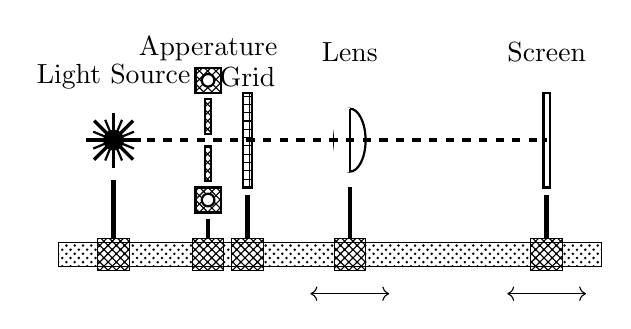
\begin{tikzpicture}
    \coordinate (S) at (0.0,0);
    \coordinate (A) at (1.2,0);
    \coordinate (G) at (1.7,0);
    \coordinate (L) at (3.0,0);
    \coordinate (I) at (5.5,0);
    \coordinate (B) at (0,-1.45);

    % Laser Symbol
    \begin{scope}[shift={(S)}, scale=0.7]
        \draw[ultra thick, fill = black] (0,0) circle (0.15);
        \draw[rotate=0, very thick] (-0.5,0) -- (0.5,0);
        \draw[rotate=90, very thick] (-0.5,0) -- (0.5,0);
        \draw[rotate=45, very thick] (-0.5,0) -- (0.5,0);
        \draw[rotate=135, very thick] (-0.5,0) -- (0.5,0);

        \draw[rotate=22.5, thick] (-0.4,0) -- (0.4,0);
        \draw[rotate=67.5, thick] (-0.4,0) -- (0.4,0);
        \draw[rotate=112.5, thick] (-0.4,0) -- (0.4,0);
        \draw[rotate=157.5, thick] (-0.4,0) -- (0.4,0);
    \end{scope}

    % % Camera/Eye
    % \begin{scope}[shift={(C)}, rotate=180]
    %     % Eye
    %     \draw[very thick] (0.5, 0.5) -- (0, 0) -- (0.5, -0.5);
    %     \draw[very thick] (0.33, -0.3) arc (-30:30:0.6);
    % \end{scope}

    % Apperature
    \begin{scope}[shift={(A)}, scale=0.4]
        \draw[thick, pattern=crosshatch] (-0.1,1.3) rectangle (0.1,0.2);
        \draw[thick, pattern=crosshatch] (-0.1,-0.2) rectangle (0.1,-1.3);

        \draw[thick, pattern=crosshatch] (-0.4,1.5) rectangle (0.4, 2.3);
        \draw[thick, pattern=crosshatch] (-0.4,-1.5) rectangle (0.4, -2.3);

        \draw[thick, fill=white] (0,1.9) circle (0.2);
        \draw[thick, fill=white] (0,-1.9) circle (0.2);
    \end{scope}

    % Grid
    \begin{scope}[shift={(G)}, scale=0.4]
        \draw[thick, pattern=grid] (-0.15,1.5) rectangle (0.15,-1.5);
    \end{scope}

    % Lens
    \begin{scope}[shift={(L)}, scale=0.5]
        %\draw[thick] (-0.3, -0.6) rectangle (0.3, 0.6);
        %\draw[dashed] (-0.5,-0.5) -- (0.5,0.5);
        %\coordinate (P1) at (0,0);
        \draw[thick] (0,0) ellipse (0.4 and 0.8);
        \filldraw[fill=white, color=white] (0,0.8) rectangle (-0.4,-0.8);
        \draw[thick] (0,0.8) -- (0,-0.8);
    \end{scope}

    % Imaging screen
    \begin{scope}[shift={(I)}, scale=0.4]
        \draw[thick] (-0.1,1.5) rectangle (0.1,-1.5);
    \end{scope}

    % Laser Path
    \draw[ultra thick, dashed] (S) -- (A) -- (G) -- (L) -- (I);

    % Optical Bench
    \draw[pattern=crosshatch dots] ($(S)+(-0.7,0.15)+(B)$) rectangle ($(I)+(0.7,-0.15)+(B)$);

    % Mounts
    \draw[pattern=crosshatch] ($(S)+(B)+(0.2,0.2)$) rectangle ($(S)+(B)-(0.2,0.2)$);
    \draw[ultra thick] ($(S)+(B)+(0,0.2)$) -- ($(S)+(0,-0.5)$);

    \draw[pattern=crosshatch] ($(A)+(B)+(0.2,0.2)$) rectangle ($(A)+(B)-(0.2,0.2)$);
    \draw[ultra thick] ($(A)+(B)+(0,0.2)$) -- ($(A)+(0,-1)$);

    \draw[pattern=crosshatch] ($(G)+(B)+(0.2,0.2)$) rectangle ($(G)+(B)-(0.2,0.2)$);
    \draw[ultra thick] ($(G)+(B)+(0,0.2)$) -- ($(G)+(0,-0.7)$);

    \draw[pattern=crosshatch] ($(L)+(B)+(0.2,0.2)$) rectangle ($(L)+(B)-(0.2,0.2)$);
    \draw[ultra thick] ($(L)+(B)+(0,0.2)$) -- ($(L)+(0,-0.6)$);

    \draw[pattern=crosshatch] ($(I)+(B)+(0.2,0.2)$) rectangle ($(I)+(B)-(0.2,0.2)$);
    \draw[ultra thick] ($(I)+(B)+(0,0.2)$) -- ($(I)+(0,-0.7)$);

    \draw[<->] ($(L)+(B)+(-0.5,-0.5)$) -- ($(L)+(B)+(0,-0.5)$) -- ($(L)+(B)+(0.5,-0.5)$);

    \draw[<->] ($(I)+(B)+(-0.5,-0.5)$) -- ($(I)+(B)+(0,-0.5)$) -- ($(I)+(B)+(0.5,-0.5)$);

    % Labels
    \node[anchor=south, yshift=15] at (S) {Light Source};
    \node[anchor=south, yshift=25] at (A) {Apperature};
    
    \node[anchor=south, yshift=16] at (G) {Grid};
    \node[anchor=south, yshift=25] at (L) {Lens};
    \node[anchor=south, yshift=25] at (I) {Screen};

\end{tikzpicture}
            %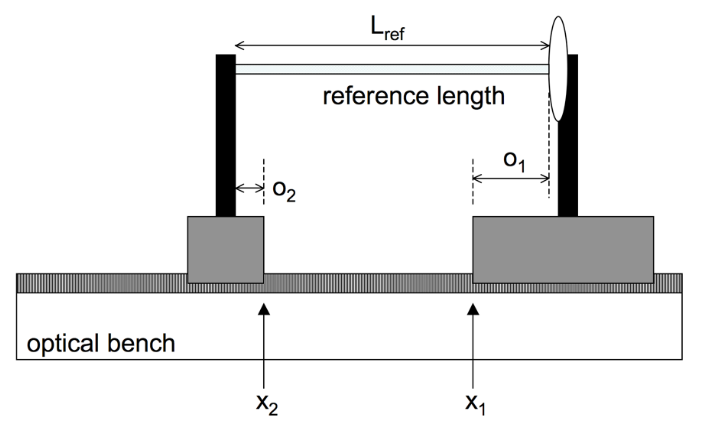
\includegraphics[width=0.8\linewidth]{figures/optical-bench.png}
            \caption{Experimental setup for measuring the focal length of a lens. This image specifically looks how how measurements wer taken using reference lengths.}
            \label{fig:expsetup}
        \end{figure}

        Proper alignment of the optical components was critical. Three primary components were used:, a light source\footnote{Exact model number and manufacturer to be recorded.}, a variable diaphram apperature, a lens mounted on vertical and horizontal translation stage, and a screen. Adjustments were first made near to the point light source to ensure the beam was aligned correctly. The screen was then progressively moved back until the image remained at the same inital point on the screen. Fine adjustments were initially made on the lamp's translation and adjustment stages with later adjustments being made on the lens mount.

        Onece a lens was placed within the mount, the lens was adjusted vertically and horizontally using translation stages until the backreflection of the lens was directly back into the bulb.

        \begin{figure}[H]
            \centering
            %\input{figures/far-field.tex}
            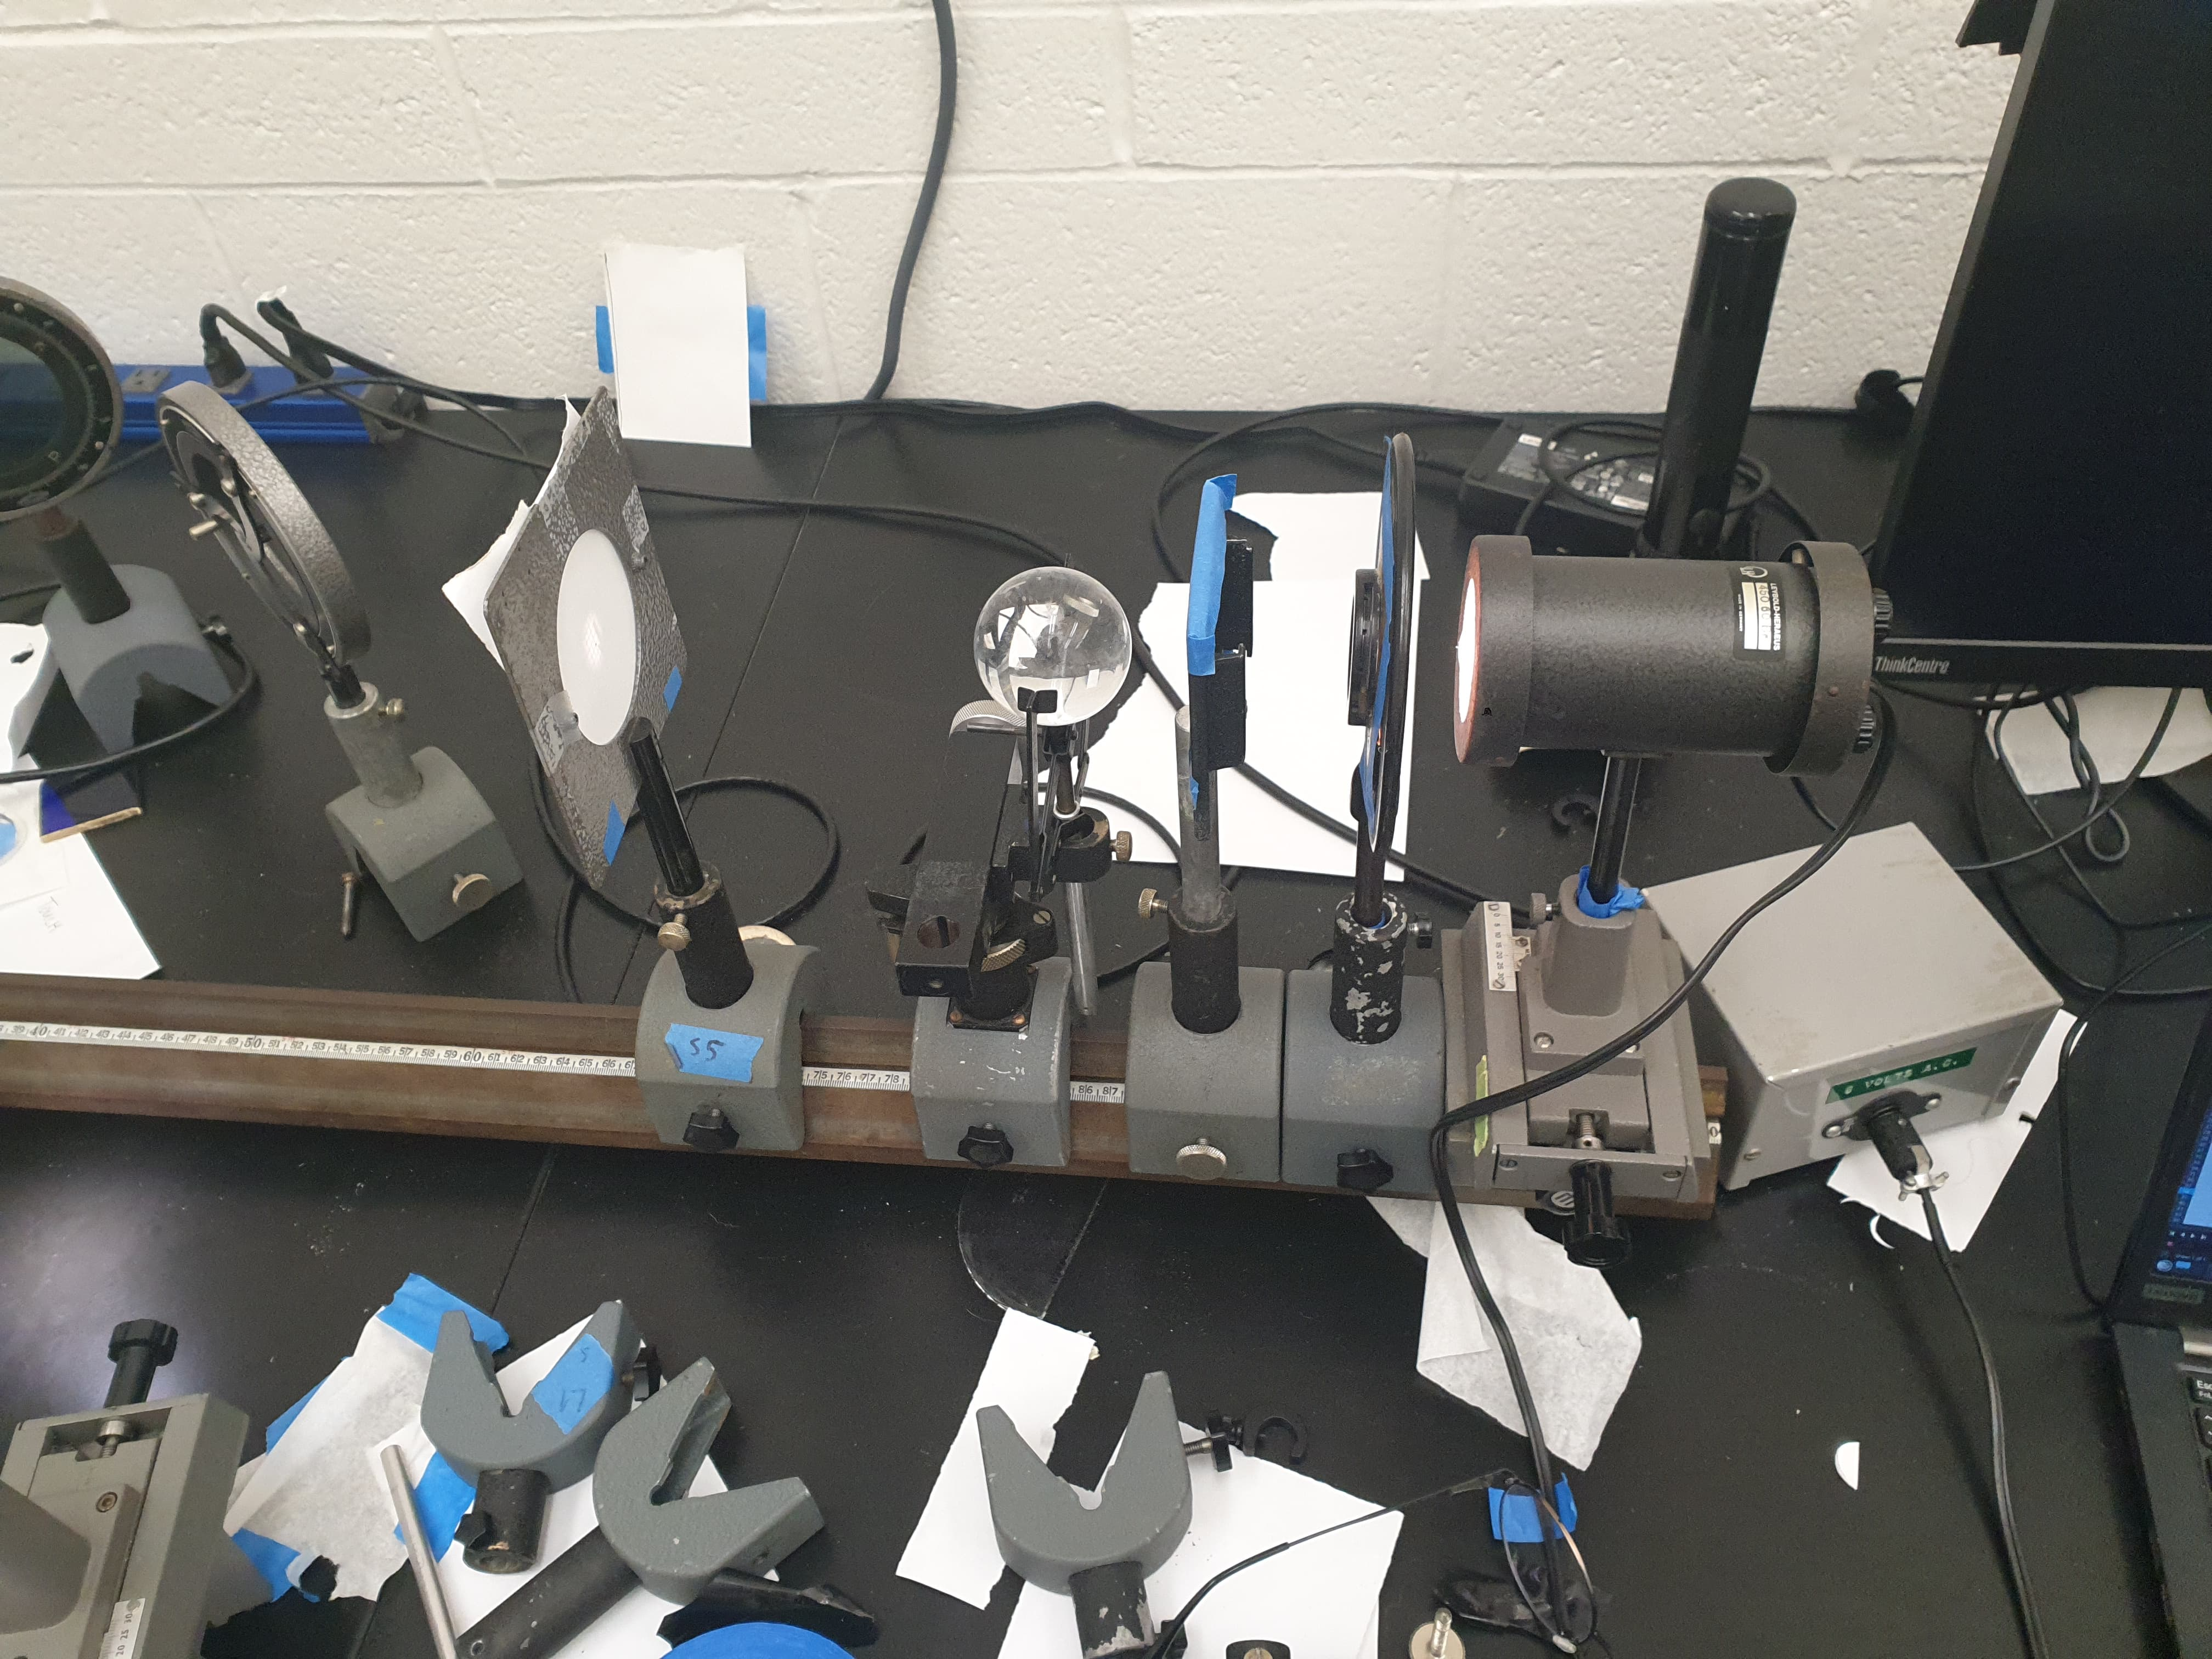
\includegraphics[width=0.8\linewidth]{figures/setup.jpeg}
            \caption{Actual experimental setup used. The lamp is positioned at the edge of the optical rail on a horizontal translation stage. Additional adjustments could be made to the bulb, though this significantly affected alignment and was difficult to tune.}
            \label{fig:realsetup}
        \end{figure}

        % Alignment Procedures  
        Initial estimates of the focal length of each lens were obtained using a far field method. The lens was placed at a distance from the light source such that the image formed was at the far field. The distance between the lens and the screen was then measured to obtain the focal length. This method was repeated for each lens to ensure consistency.
        % \begin{enumerate}
        %     \item The lamp was positioned behind a diaphragm with a small aperture to produce a collimated beam.
        %     \item A screen was placed at a short distance from the diaphragm to check for alignment by marking the central light spot.
        %     \item The lens was positioned approximately 7 cm from the diaphragm, and its angle was adjusted to retro-reflect light back through the aperture.
        %     \item The screen was moved about 1 m away to observe the far-field focus, ensuring the beam remained centered.
        %     \item Fine adjustments were made iteratively to confirm proper alignment.
        % \end{enumerate}

        An additional grid was placed before the lens to measure geometric magnification and any distortions introduced by the lens. Given there was some distortion despite multiple realignment attempts, a $3\times3$ unit block of values was recorded as well as multiple readings for each configuration.

        \begin{figure}[H]
            \centering
            %\input{figures/far-field.tex}
            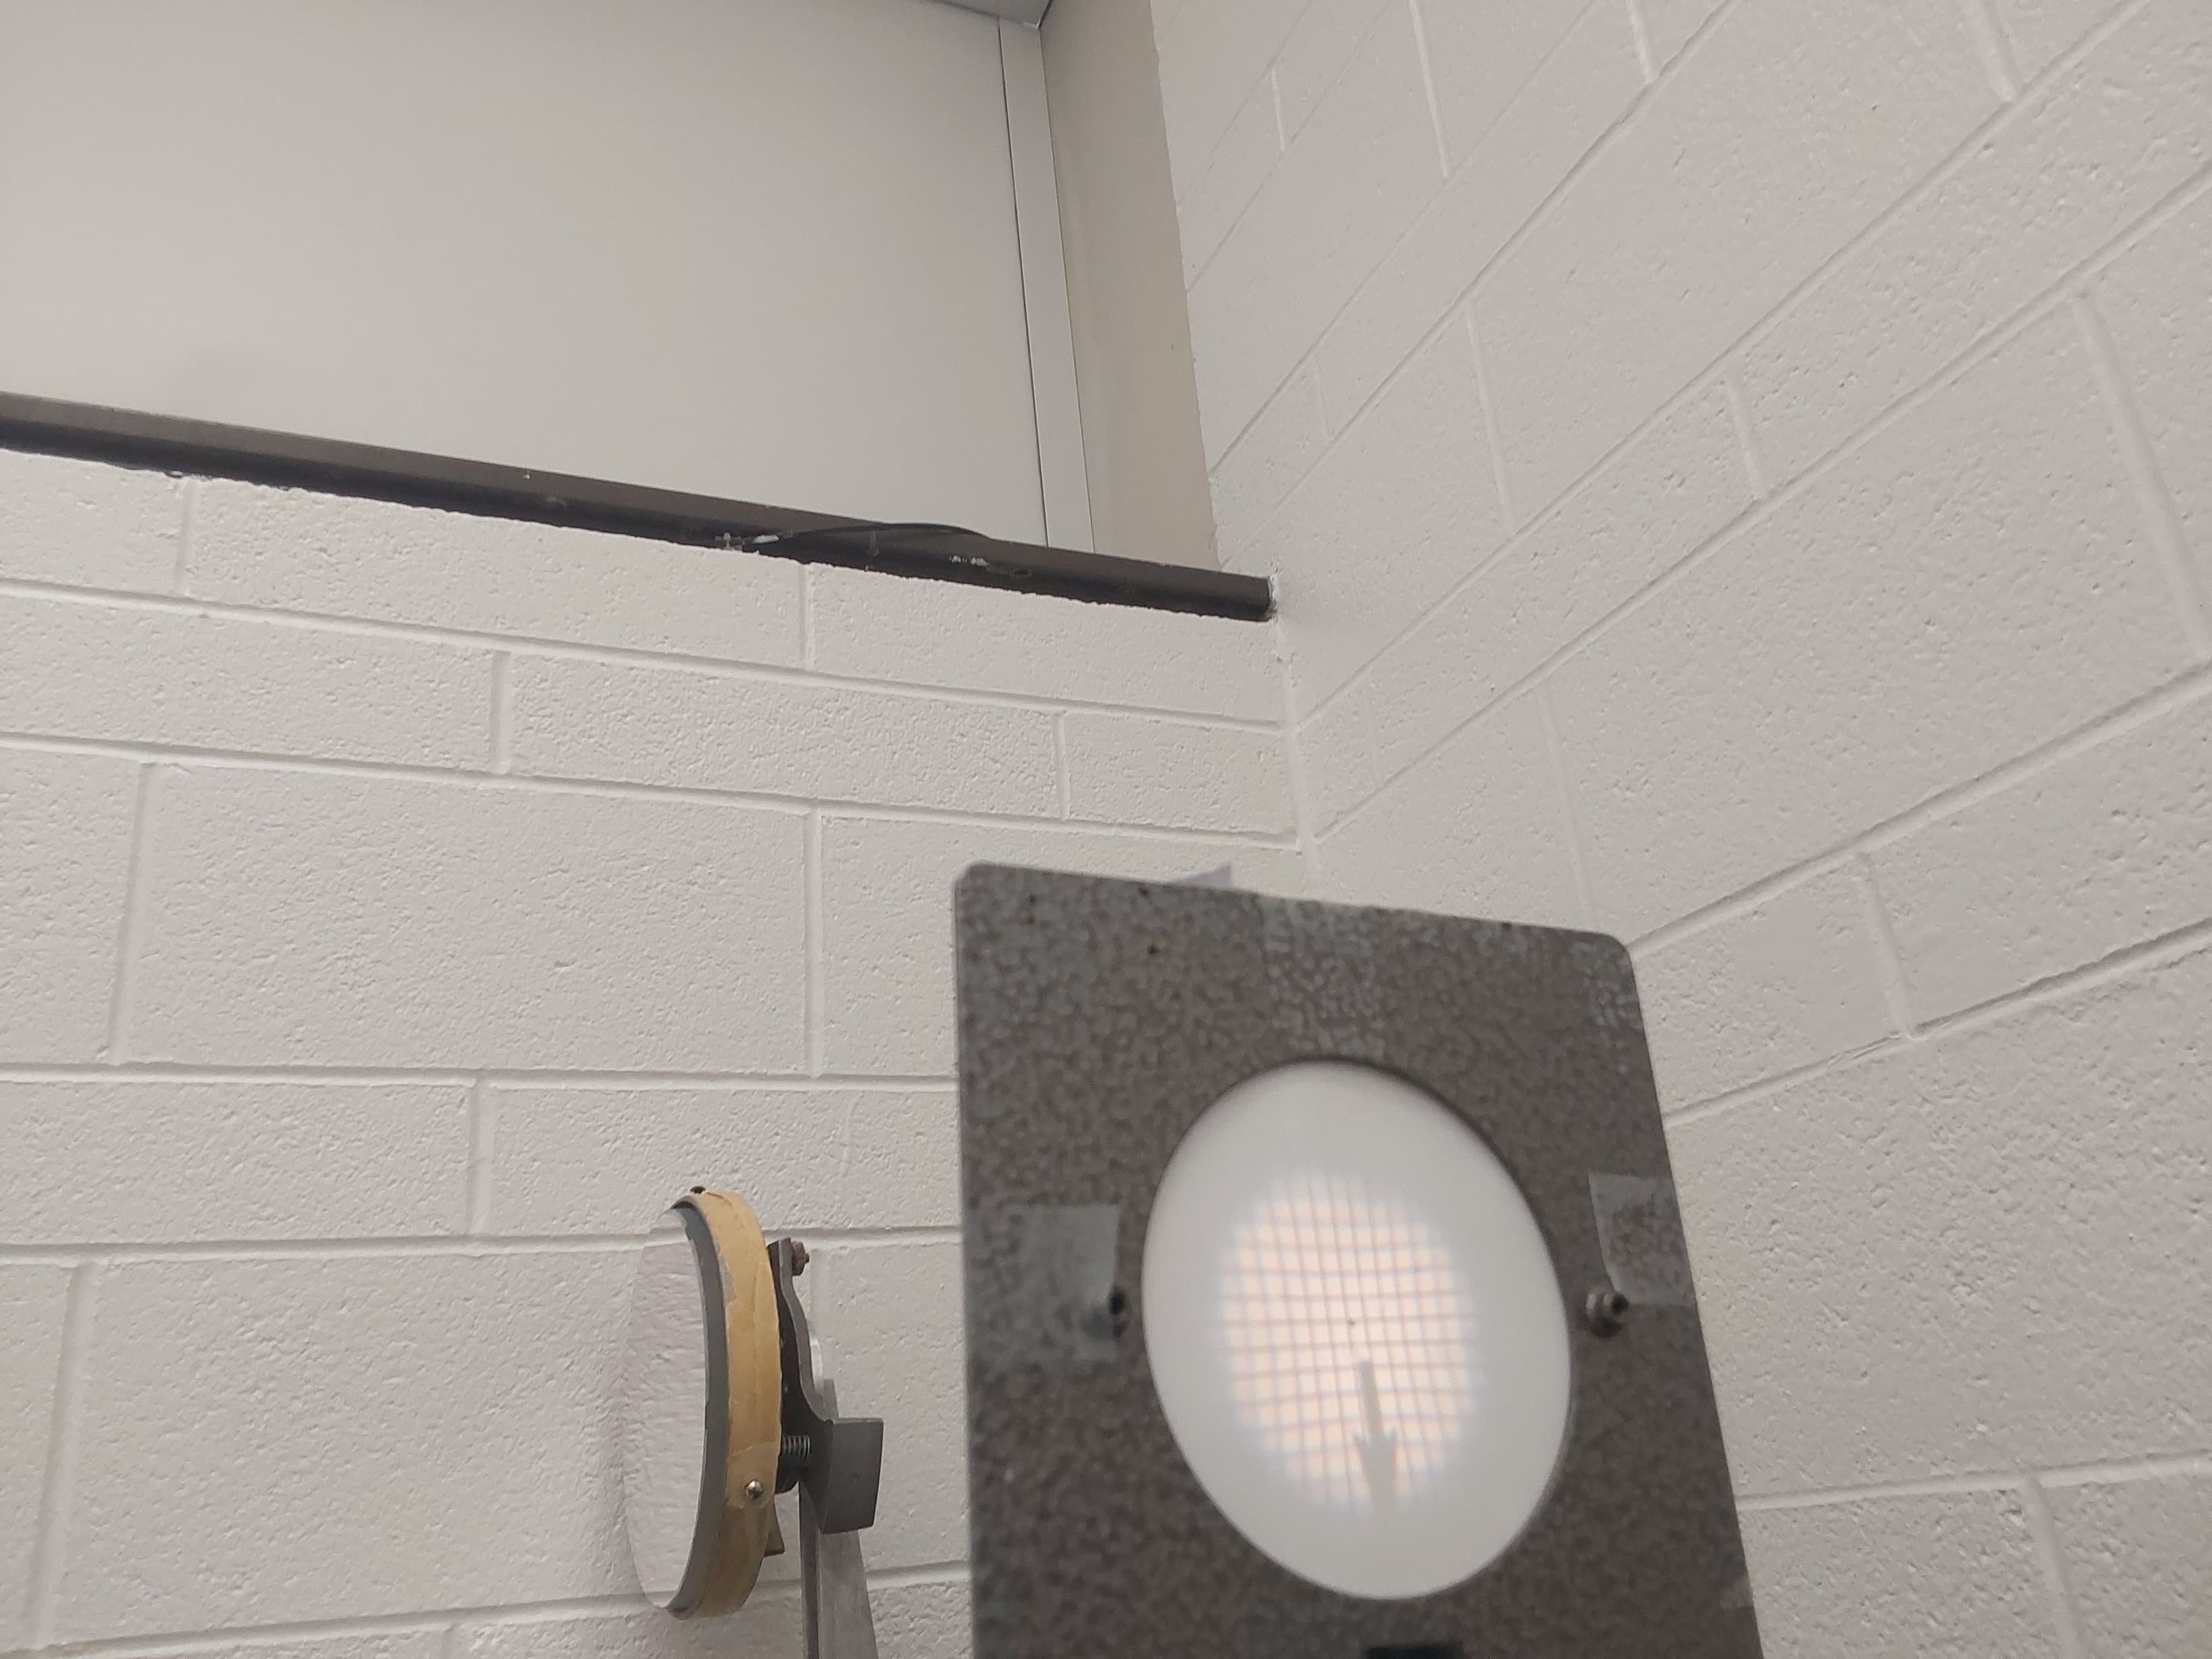
\includegraphics[width=0.8\linewidth]{figures/grid.jpeg}
            \caption{$3\times3$ grid points used to mitigate distorition effects present.}
            \label{fig:grid}
        \end{figure}

        This reduced uncertainty in measurement from distortion effects because any distorition effects present were averaged out across the grid. Therefore, the average of the $3\times3$ grid was used to calculate the distance between the grid points. 

        % \subsection{Focal Length Estimation}
        % The focal length of each lens was estimated through two methods:
        % \begin{enumerate}
        %     \item Measuring the image distance when the lens was far from the light source.
        %     \item Using the lensmaker's equation:
        %     \begin{equation}
        %         f = \frac{R}{2(n-1)}
        %     \end{equation}
        %     where $R$ is the radius of curvature and $n$ is the refractive index of the lens material.
        % \end{enumerate}

        For data collection post alignment, the position of the source was fixed for all measurements. The lens was then placed at $5$ different locations on the optical bench. At each location, $3$ measurements were taken by moving the screen to obtain a sharp image of the grid, this image distance was then recorded. This procedure was repeated for a variety of lenses, namely a plano-convex lens, a biconvex lens, a concave-convex lens, and a spherical lens. 
        
        The magnification was calculated by measuring the grid line spacing in the image. The process was repeated for a range of object and image distances. Data was verified by checking consistency with \eqref{eqn:thinlens}.

        For thicker lenses, additional measurements were taken to determine whether the thin lens approximation remained valid. The locations of the front and back principal planes were estimated, and deviations from the ideal thin lens behavior were analyzed.

    \section{Results \& Analysis}
            The primary two lenses compared in this analysis are the thin biconvex lens and the thick biconvex lens. Performating a linear fit to the thin lens equation yields a naive approximation of the focal length in figure \ref{fig:thinlens-inv}. This was then used to do additional fits utilizing the thin lens equation \eqref{eqn:thinlens} and the thick lens equation \eqref{eqn:thicklens}. 

            \begin{figure*}
                \centering
                \begin{subfigure}[b]{0.24\linewidth}
                    \centering
                    %\input{figures/thinlens.tex}
                    \includegraphics[width=\linewidth]{figures/Biconvex-inv.png}
                    \caption{Fit to $q^{-1} = f^{-1} -  p^{-1}$ with the objective fit parameter being $f^{-1}$. It was found that $f_\text{thin} = 17.9\pm0.3$ with $\chi^2_\text{red} = 0.03$.}
                    \label{fig:biconvex-inv}
                \end{subfigure}
                \begin{subfigure}[b]{0.24\linewidth}
                    \centering
                    %\input{figures/thinlens.tex}
                    \includegraphics[width=\linewidth]{figures/Thick-Biconvex-inv.png}
                    \caption{Fit to $q^{-1} = f^{-1} -  p^{-1}$ with the objective fit parameter being $f^{-1}$. It was found that $f_\text{thick} = 9.7\pm0.4$ with $\chi^2_\text{red} = 0.04$.}
                    \label{fig:thickbiconvex-inv}
                \end{subfigure}
                \begin{subfigure}[b]{0.24\linewidth}
                    \centering
                    %\input{figures/thinlens.tex}
                    \includegraphics[width=\linewidth]{figures/Biconvex-thin.png}
                    \caption{Fit to $q = (f^{-1} -  p^{-1})^{-1}$ with the objective fit parameter being $f^{-1}$. It was found that $f_\text{thin} = 18.0\pm0.4$ with $\chi^2_\text{red} = 90$.}
                    \label{fig:biconvex-thin}
                \end{subfigure}
                \begin{subfigure}[b]{0.24\linewidth}
                    \centering
                    %\input{figures/thinlens.tex}
                    \includegraphics[width=\linewidth]{figures/Thick-Biconvex-thin.png}
                    \caption{Fit to $q = (f^{-1} -  p^{-1})^{-1}$ with the objective fit parameter being $f^{-1}$. It was found that $f_\text{thick} = 9.5 \pm 0.2$ with $\chi^2_\text{red} = 18$.}
                    \label{fig:thickbiconvex-thin}
                \end{subfigure}
                \caption{Fitting to the thin lens equation. Clearly, \figref{fig:biconvex-inv} and \figref{fig:thickbiconvex-inv} show a deviation. However, \figref{fig:biconvex-thin} does not deviate as much compared to \figref{fig:thickbiconvex-thin}. Goodness-of-fit tests for \figref{fig:biconvex-inv} and \figref{fig:thickbiconvex-inv} show that the data is overfit. However, \figref{fig:biconvex-thin} and \figref{fig:thickbiconvex-thin} indicate an underfitting.}
                \label{fig:thinlens}
            \end{figure*}

            Performing a fit to the thick lens equation \eqref{eqn:thicklens} yields a better approximation of the focal length. Both the thin and thick biconvex lenses benifitted from utilizing the full equation. This is evident in \figref{fig:biconvex-thicklens} and \figref{fig:thickbiconvex-thicklens}.

            \begin{figure}[H]
                \centering
                \includegraphics[width=0.7\linewidth]{figures/Biconvex-thick.png}
                \caption{Fit to the thick lens equation \eqref{eqn:thicklens} for a thin biconvex lens with fit parameters $f$, $f_p$, and $b_p$. The found parameters are $f = 17.0 \pm 0.4$, $f_p = 3.8 \pm 0.7$ and  $b_p = -3.1 \pm 1.0$ with $\chi^2_{\text{red}} = 0.2$. Goodness-of-fit tests show that the data is overfitting, however, residuals show no significant pattern indicating that this is still a good approximation.}
                \label{fig:biconvex-thicklens}
            \end{figure}

            Clearly a much better representation of the data is found in \figref{fig:biconvex-thicklens}. However, a $\chi^{2}_\text{red} = 0.2$ indicates that the data is overfit. Therefore, one may conclude that the thin lens equation is sufficient for a thin biconvex lens as expected. This is furhter reflected with both found focal lengths being similar $f_\text{thin} = 18.0\pm0.4$ and $f_\text{thick} = 17.0\pm0.4$.

            One may further test the thick biconvex lens as seen in \figref{fig:thickbiconvex-thicklens} to see that this yields a much better approximation of the data.

            \begin{figure}[H]
                \centering
                \includegraphics[width=0.7\linewidth]{figures/Thick-Biconvex-thick.png}
                \caption{Fit to the thick lens equation \eqref{eqn:thicklens} for a thin biconvex lens with fit parameters $f$, $f_p$, and $b_p$. The found parameters are $f = 9.2 \pm 1.0$, $f_p = 3.8 \pm 0.7$ and  $b_p = -3.1 \pm 1.0$ with $\chi^2_{\text{red}} = 0.5$. Goodness-of-fit tests is within an acceptable range with residuals showing no significant pattern indicating that the equation is representative of the data.}
                \label{fig:thickbiconvex-thicklens}
            \end{figure}

            Clearly, the thick lens equation is a better represenation of the data. This is reflected in a $\chi^{2}_\text{red} = 0.5$ indicating that the data is fit within an acceptable range though slightly overfit. However, it should be noted that the uncertainty in the focal length is significantly larger when fitting with the thick lens equation. This is likely because of measurement error during data collection as indicated from the large uncertainty as $p\rightarrow0$. Therefore, one may conclude that the thin lens equation is a not a good approximation for the thick biconvex lens and thus the thick lens equation should be used.

            Additionally, the convex-concave and concave-convex lenses were also analyzed. The results of these lenses are tabulated in Tab.{tab:lens}. 

            \begin{table}[H]
                \begin{tabular}{c|c|c|c|c}
                    \hline\hline
                    \multirow{2}{*}{Lens Type} & \multicolumn{2}{c}{Thin Lens Equation} & \multicolumn{2}{c}{Thick Lens Equation} \\
                     & $f$ & $\chi^2_{\text{red}}$ & $f$ &$\chi^2_{\text{red}}$\\
                    \hline
                    Biconvex & $18.0 \pm 0.4$ & $90$ & $17.0 \pm 0.4$ & $0.2$\\
                    Thick Biconvex & $9.5 \pm 0.2$ & $18$ & $9.2 \pm 1.0$ & $0.5$ \\
                    Convex-Concave & $22.9 \pm 0.2$ & $6$ & $53.3 \pm 10.0$ & $0.03$\\
                    Concave-Convex & $22.9 \pm 0.2$ & $6$ & $33.5 \pm 8.0$ & $0.2$\\
                    \hline\hline
                \end{tabular}
                \caption{Summary of the data for the four lenses analyzed for both the thin and thick lens equations. The data was fit to boeth \eqref{eqn:thinlens} and \eqref{eqn:thicklens} to the focal length of the lens computationally.}
                \label{tab:lens}
            \end{table}

            An interesting result is that the convex-concave and concave-convex lenses have the same focal length when using the thin lens equation but differ drastically when using the thick lens equation. This is an area which should be investigated in future analysis.

            It is also generally interesting that the thin lens equation still differs significantly. This is summarized in \figref{fig:thincompare} and \figref{fig:thickcompare}.

            \begin{figure}[H]
                \centering
                \begin{subfigure}[b]{0.49\linewidth}
                    \centering
                    %\input{figures/thinlens.tex}
                    \includegraphics[width=0.9\linewidth]{figures/Biconvex.png}
                    \caption{Fit of thick and thin lens equations compared for a thin biconvex lens. }
                    \label{fig:thin-compare}
                \end{subfigure}
                \begin{subfigure}[b]{0.49\linewidth}
                    \centering
                    %\input{figures/thinlens.tex}
                    \includegraphics[width=0.9\linewidth]{figures/Thick-Biconvex.png}
                    \caption{Fit of thick and thin lens equations compared for a thick biconvex lens. }
                    \label{fig:thick-compare}
                \end{subfigure}
                \caption{Illustration of difference in thick and thin lens equations. Clearly in \figref{fig:thin-compare} the deviation is larger than in \figref{fig:thick-compare}. This is expected as the thin lens equation is a simplification of the thick lens equation.}
                \label{fig:thincompare}
            \end{figure}

            It is worth noting that these deviations are primarily in the limit as $p\rightarrow0$. This may be because, as the distance to the image is decreased, the lens is no longer able to focus the light as well. Additionally, this may be a result of data aquisition error as at lower values of $p$ the focal point is harder to find visually.

        \subsection{Chromatic Aberrations}

            Data points taken for triprism calibration are shown in \figref{fig:chromatic-He} and \figref{fig:chromatic-H}. These were both fit to \eqref{eqn:triprism} to obtain the calibration constants. The spectroscope constant was provided $\lambda_0 = 284.6 \pm 0.4\,\text{nm}$.

            \begin{figure}[H]
                \centering
                \begin{subfigure}[b]{0.49\linewidth}
                %\input{figures/chromatic.tex}
                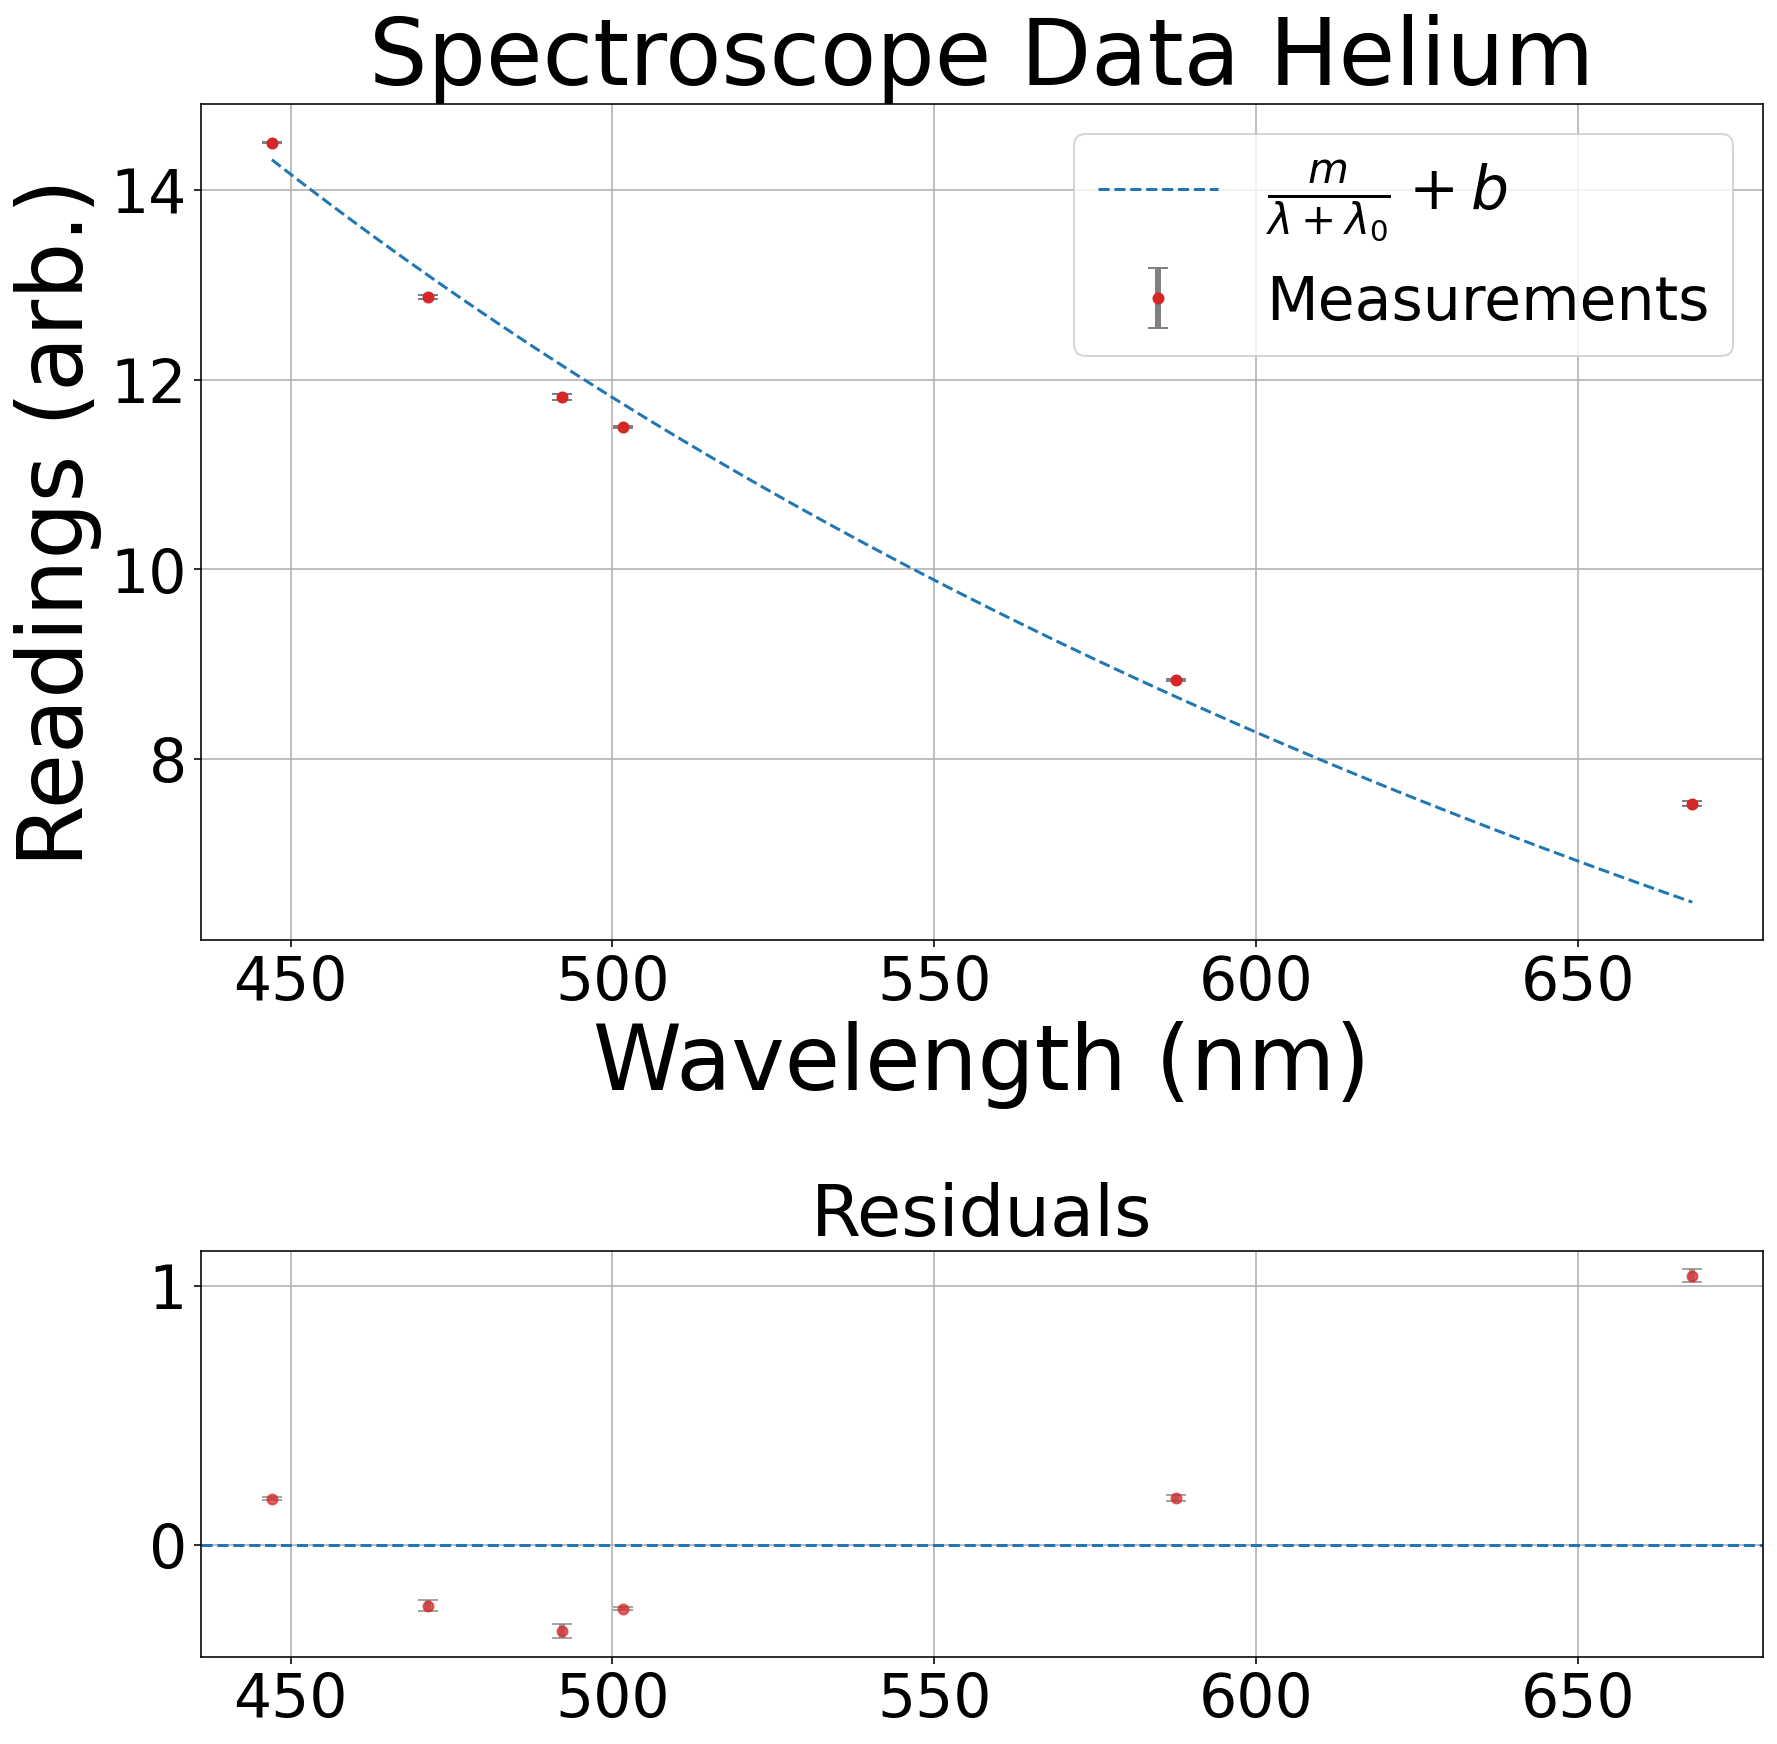
\includegraphics[width=\linewidth]{figures/spec-he.png}
                \caption{Fit parameters $m = 1000\pm700$, $\b=-9\pm 1$, $\chi^2_{\text{red}} = 1248$.}
                \label{fig:chromatic-He}
                \end{subfigure}
                \begin{subfigure}[b]{0.49\linewidth}
                \centering
                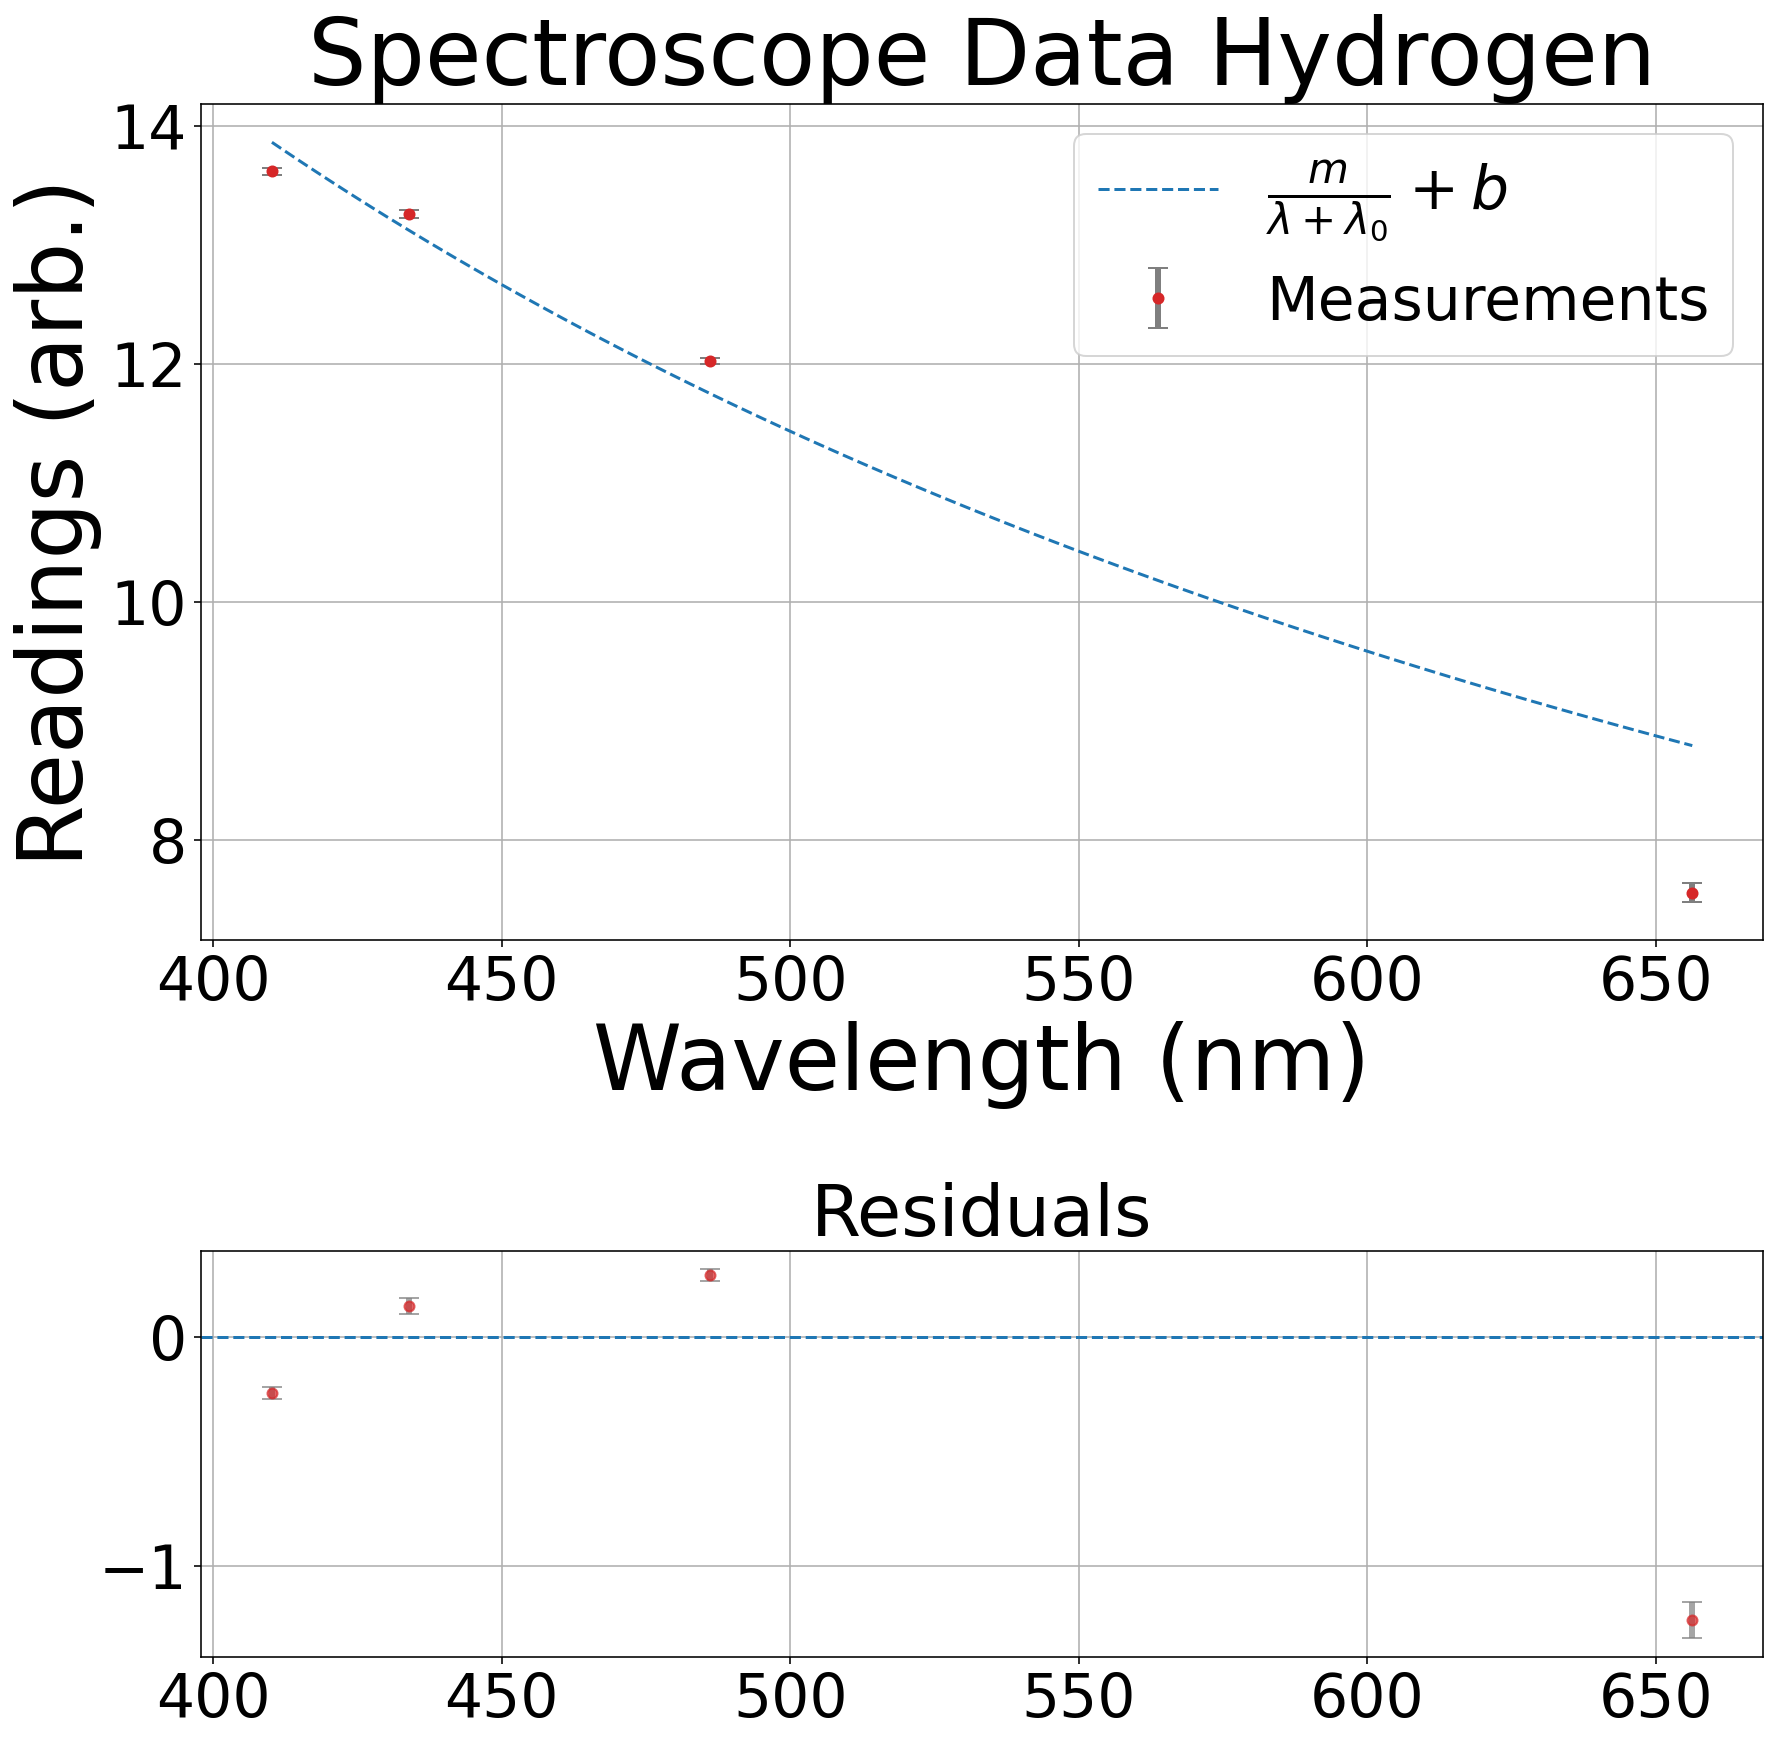
\includegraphics[width=\linewidth]{figures/spec-h.png}
                \caption{Fit parameters $m = 500\pm100$, $\b=-0.3\pm 2$, $\chi^2_{\text{red}} = 230$. }
                \label{fig:chromatic-H}
                \end{subfigure}
                \caption{Calibration curves for the triprism spectroscope using a $\text{He}$ (\figref{fig:chromatic-He}) and $\text{H}$ sample (\figref{fig:chromatic-He}). The data was fit to \eqref{eqn:triprism} to obtain the calibration constants. Residuals show some pattern indicating an under estimation of uncertainties. The high $\chi^2_\text{red}$ indicates that the data is not a good fit.}
            \end{figure}

            Clearly, both fits show some pattern in the residuals indicating that the uncertainties were underestimated. However, qualitatively, this fits do indeed look decent. However, it should be noted that some odd observations were observed during data collection. Namely, multiple additional spectral lines were visable in both the $\text{He}$ and $\text{H}$ samples\footnote{This phenomena was also observed by the technical staff}. Overall, given the high $\chi^2_\text{red}$ values, it is likely that the data is not a good fit and hence futher investigation and calibration of the triprism spectroscope is needed.
    
    \section{Conclusion}
        This study effectively quantitatively verified the thin lens equation for most of the lenses studied. The experimental setup consisted of an optical rail/bench with a lamp, adjustable iris apperature, lens holder on vertical (and horizontal) translation stage, and a screen. Uncertainties were estimated using both statistical and systematic methods. with the later being from the gradations on measurement tools and the former being from the standard deviation of multiple readings.
        
        Additional measurements were taken to characterize the chromatic aberrations in a plano-convex lens. The calibration of the triprism spectroscope for both Hydrogen and Helium were both very suboptimal with goodness-of-fit tests $\chi^2_\text{red}=230$ and $\chi^2_\text{red}$ respectively indicating a massive underestimation of uncertainties and underfitting to the data. There was also interesting observations of multiple unexpected spectral lines in both the Hydrogen and Helium samples. This phenomena was also observed by the technical staff and with the cause not being obvious. As a result, this data was not used for analysis in conjuction with an insifficult amount of data being collected for the Green light source. This is an area which would benifit from further investigation. Specifically, the spectral lines should be investigated to see if they are indeed real or a result of some interesting phenomena occurring within the spectroscope.

        It was found that, the thin lens equation was only useful as an approximation for all the lens used. However, for thin lenses, the devations were less aggregious. For the thin biconvex lens, the thin lens equation was a good approximation with a focal length of $f_\text{thin} = 18.0\pm0.4$ and $f_\text{thick} = 17.0\pm0.4$. Though there is a difference in the focal length, the overall deviation is small as evident from \figref{fig:thin-compare}. The same is not true for the thick biconvex lens where the thin lens equation was not a good approximation. The focal length of the thick biconvex lens was found to be $f_\text{thin} = 9.5\pm0.2$ and $f_\text{thick} = 9.2\pm1.0$. Though these values are similar, the deviation in the fitted equations is significant as seen in \figref{fig:thick-compare}. The drastic difference in the uncertainty 
        
        An additional anecdote is the fact that the convex-concave and concave-convex lenses had the same focal length when using the thin lens equation but differed drastically when using the thick lens equation. This is quite curious as it indicates that the thin lens equation is not a good approximation for these lenses despite the lenses themselves being thin. This is because one would expect that the focal length would differ given the reversal of the lens. This is an area which would benifit from further investigation. 

        In conclusion, it was found that the thin lens equation was sufficient for thin lenses when the image $p$ was not small. However, for all data lenses analyzed, the thick lens equation served as a better representation of the data. However, it must be noted that this may be due to an overfitting (in the case of thin lenses) as goodness-of-fit tests in Tab.\ref{tab:lens} are low for the thin lenses analyzed. 
        Further investigations may be fruitful in this area. One effect not studied in this report is the into the effect of the curvature of the lens on the focal length and the validity of both the thick and thin lens equations as this may be the cause of the devations found in the case of the Concave-Convex lens.
    % Line to seperate report content from acknowledgements and references
\onecolumngrid
\begin{center}
    \vspace{0.8cm}
    \noindent\rule{0.9\textwidth}{0.5pt}
\end{center}

\begin{acknowledgments}
    The author would like to thank Prof. \advname (Supervising Professor) and \taname (Teaching Assistant) for their guidence and support throughout the experiment. Moreover, the author would like to further acknowledge the support of the lab technician team L. Avramidis and P. Scolieri for their assistance in debugging issues that arose with the triprism spectroscope. Finally, the support of author experimentors in MP250 should be acknowledged as they provided valuable feedback and suggestions during the experiment.
\end{acknowledgments}

\bibliography{references}

% \appendix
% \section{Appendix}

% \subsection{Raw Data}

% \subsection{Code}

\end{document}